\documentclass[12pt,a4paper]{article}
\usepackage[utf8]{inputenc}
\usepackage[T1]{fontenc}
\usepackage{amsmath}
\usepackage{amsfonts}
\usepackage{amssymb}
\usepackage{graphicx}
\usepackage[width=0.00cm, left=3.00cm, right=2.00cm, top=3.00cm, bottom=2.00cm]{geometry}
\usepackage{booktabs}
\usepackage{pgfplots}
\usepackage{adjustbox}
\title{Lista 2}
\date{}
\begin{document}
	\begin{center}
		\includegraphics[width=100px]{Logo.png}\\
		\textsc{Universidade Federal de Pernambuco\\
			Centro de Ciências Sociais Aplicadas\\
			Departamento de Ciências Contábeis e Atuariais\\}
		\vspace{5cm}
		\huge Lista 2\\ \normalsize
		\vspace{4cm}
	\end{center}
	\newpage
	\textbf{1. Hepatite}
	\vspace{0.5cm}\\
	Um estudo clínico aleatorizado com 29 indivíduos foi realizado para investigar o efeito da terapia com esteroide no tratamento de hepatite viral aguda.
	\begin{center}
		\small{Tabela 1: Tempos de sobrevivência observados no estudo de hepatite.}\\
		\begin{tabular}{|c|c|}\hline
			\textbf{Grupo} & \textbf{Tempo de Sobrevivência (em Semanas)}\\ \hline
			\textbf{Controle} & 1+, 2+, 3, 3, 3+, 5+, 5+, 16+, 16+, 16+, 16+, 16+, 16+, 16+, 16+\\ \hline
			\textbf{Esteroide} & 1, 1, 1, 1+, 4+, 5, 7, 8, 10, 10+, 12+, 16+, 16+, 16+\\ \hline
		\end{tabular}
		\vspace{1cm}\\
	\end{center}
	\textbf{1.1 Histograma dos dados}
	\begin{center}
		\vspace{1cm}
		\textbf{Histograma de Eventos Grupo Controle}
		\resizebox{300px}{!}{
			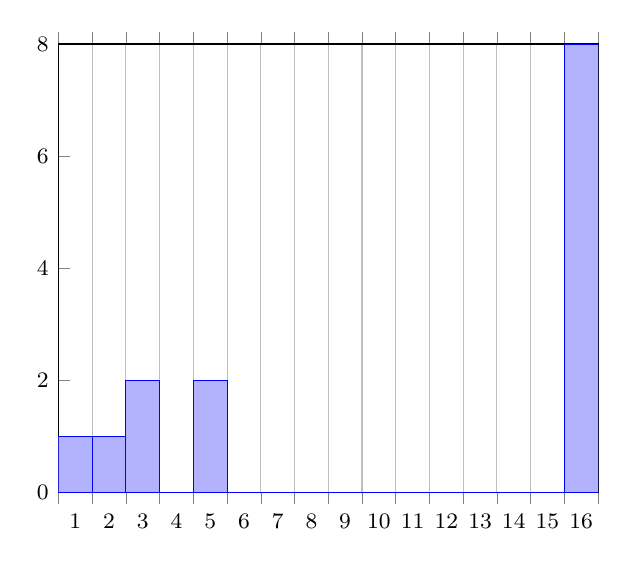
\begin{tikzpicture}
			\tikzstyle{every node}=[font=\footnotesize]
			\begin{axis}[ybar interval, ymin=0, ymax=8, xmin=1, xmax=17]
			\addplot coordinates {(1,1) (2,1) (3, 2) (4,0) (5,2) (6,0) (7,0) (8,0) (9,0) (10,0) (11,0) (12,0) (13,0) (14,0) (15,0) (16,8) (17,0)};
			\end{axis}
			\end{tikzpicture}
		}
		\vspace{1cm}\\
		\textbf{Histograma de Sobrevivência Grupo Controle}
		\resizebox{300px}{!}{
		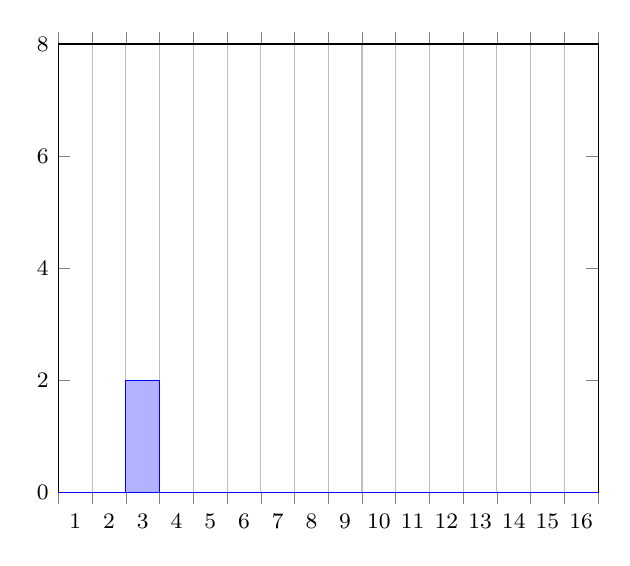
\begin{tikzpicture}
			\tikzstyle{every node}=[font=\footnotesize]
			\begin{axis}[ybar interval, ymin=0, ymax=8, xmin=1, xmax=17]
			\addplot coordinates {(1,0) (2,0) (3, 2) (4,0) (5,0) (6,0) (7,0) (8,0) (9,0) (10,0) (11,0) (12,0) (13,0) (14,0) (15,0) (16,0) (17,0)};
			\end{axis}
		\end{tikzpicture}
		}
		\vspace{1cm}\\
		\textbf{Histograma de Censuras Grupo Controle}
		\resizebox{300px}{!}{
			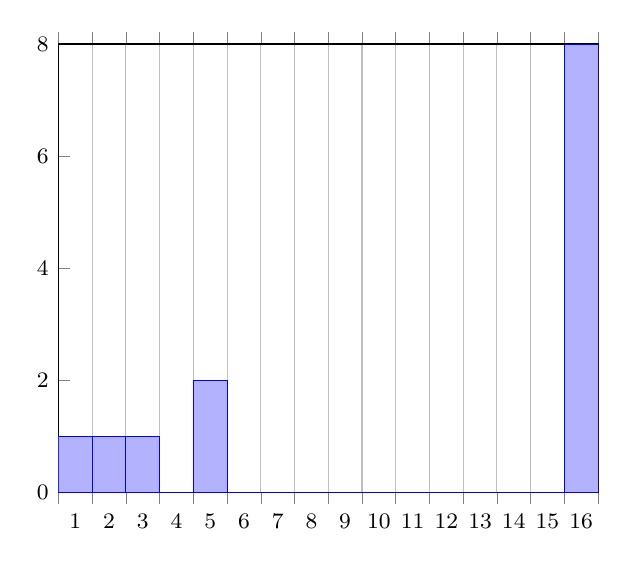
\begin{tikzpicture}
			\tikzstyle{every node}=[font=\footnotesize]
			\begin{axis}[ybar interval, ymin=0, ymax=8, xmin=1, xmax=17]
			\addplot coordinates {(1,1) (2,1) (3, 1) (4,0) (5,2) (6,0) (7,0) (8,0) (9,0) (10,0) (11,0) (12,0) (13,0) (14,0) (15,0) (16,8) (17,0)};
			\end{axis}
		\end{tikzpicture}
		}
		\vspace{1cm}\\
		\textbf{Histograma de Eventos Grupo Esteroide}
		\resizebox{300px}{!}{
			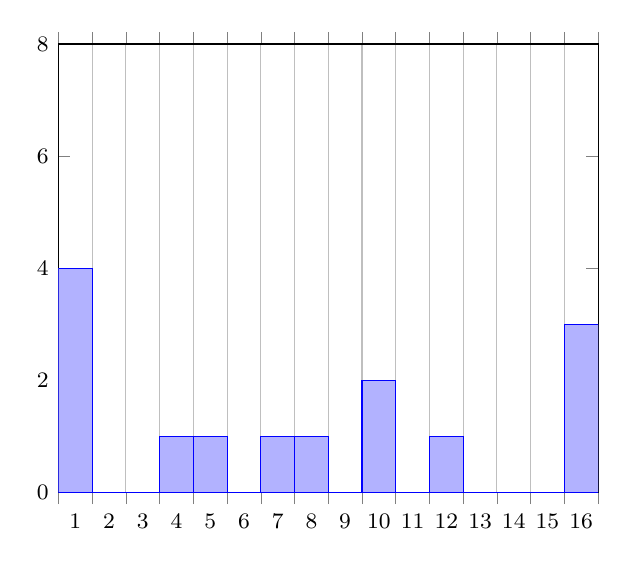
\begin{tikzpicture}
			\tikzstyle{every node}=[font=\footnotesize]
			\begin{axis}[ybar interval, ymin=0, ymax=8, xmin=1, xmax=17]
			\addplot coordinates {(1, 4) (2,0) (3,0) (4,1) (5,1) (6,0) (7,1) (8,1) (9,0) (10,2) (11,0) (12,1) (13,0) (14,0) (15,0) (16,3) (17,0)};
			\end{axis}
			\end{tikzpicture}
		}	
		\vspace{1cm}\\
		\textbf{Histograma de Sobrevivência Grupo Esteroide}
		\resizebox{300px}{!}{
		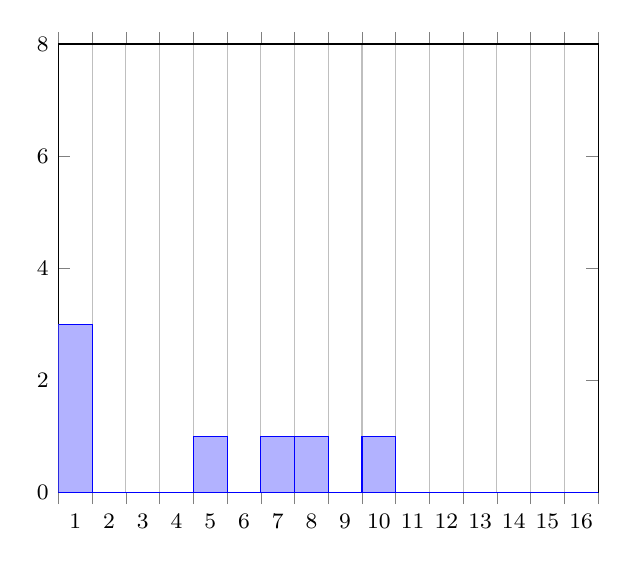
\begin{tikzpicture}
			\tikzstyle{every node}=[font=\footnotesize]
			\begin{axis}[ybar interval, ymin=0, ymax=8, xmin=1, xmax=17]
			\addplot coordinates {(1, 3) (2,0) (3,0) (4,0) (5,1) (6,0) (7,1) (8,1) (9,0) (10,1) (11,0) (12,0) (13,0) (14,0) (15,0) (16,0) (17,0)};
			\end{axis}
		\end{tikzpicture}
		}
	\vspace{1cm}\\
	\textbf{Histograma de Censuras Grupo Esteroide}
	\resizebox{300px}{!}{
		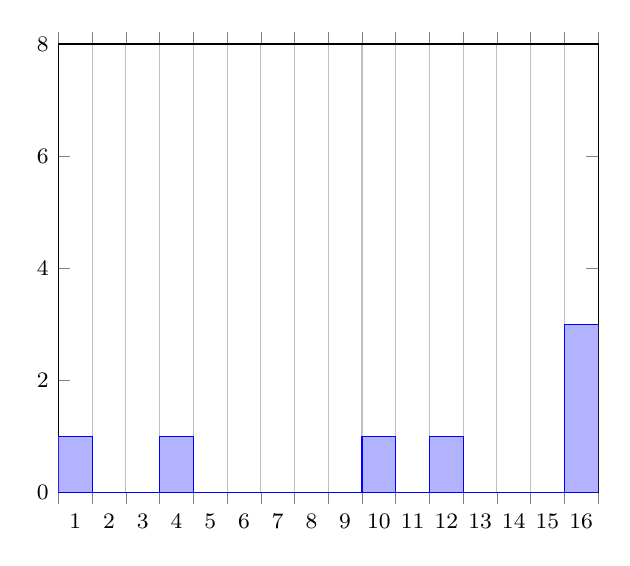
\begin{tikzpicture}
			\tikzstyle{every node}=[font=\footnotesize]
			\begin{axis}[ybar interval, ymin=0, ymax=8, xmin=1, xmax=17]
			\addplot coordinates {(1, 1) (2,0) (3,0) (4,1) (5,0) (6,0) (7,0) (8,0) (9,0) (10,1) (11,0) (12,1) (13,0) (14,0) (15,0) (16,3) (17,0)};
		\end{axis}
		\end{tikzpicture}
		}	
	\end{center}
	\vspace{1cm}
	Os histogramas de sobrevivência de ambos os grupos apresentam um número bastante reduzido de observações o que torna a modelagem dos dados mais complexa. O histograma de sobrevivência do grupo controle é especialmente complexa, já que durante o período de estudo só apresenta uma barra, significando que em todo o período de estudo em apenas 1 dos meses se observou mortes relacionadas a causa de interesse em nosso estudo, portanto a informação adicional das censuras é interessante para complementar a curva e ajudar na modelagem dos dados. Em ambos os casos dos histogramas de sobrevivência, a mortalidade parece apresentar uma maior incidência no início do período que depois se estabiliza, já nos histogramas dos eventos o grupo controle parece um crescimento exponencial, enquanto o grupo esteroide aparenta uma curva cíclica.
	\vspace{1cm}\\
	\textbf{1.2.1 Estimador de Kaplan-Meier}\\
	\begin{center}
		\resizebox{\linewidth}{!}{
		\begin{tabular}{ccccccc}\midrule
			\multicolumn{7}{c}{\textbf{Grupo Controle}}\\ \midrule 
			Tempo & Nº Risco & Eventos & Sobrevivência & Erro Padrão & IC$_{95\%}$ inferior & IC$_{95\%}$ superior\\ \midrule 
			3 & 13 & 2 & 0.846 & 0.100 & 0.671 & 1.000\\ \midrule
		\end{tabular}
		}
		\vspace{1cm}\\
		\resizebox{\linewidth}{!}{
		\begin{tabular}{ccccccc}\midrule
			\multicolumn{7}{c}{\textbf{Grupo Esteroide}}\\ \midrule
			Tempo & Nº Risco & Eventos & Sobrevivência & Erro Padrão & IC$_{95\%}$ inferior & IC$_{95\%}$ superior\\ \midrule
			1 & 14 & 3 & 0.786 & 0.110 & 0.598 & 1.000\\ \midrule
			5 & 9 & 1 & 0.698 & 0.128 & 0.488 & 0.999\\ \midrule
			7 & 8 & 1 & 0.611 & 0.138 & 0.392 & 0.952\\ \midrule
			8 & 7 & 1 & 0.524 & 0.143 & 0.306 & 0.896\\ \midrule
			10 & 6 & 1 & 0.437 & 0.144 & 0.229 & 0.832\\ \midrule
		\end{tabular}
		}
		\vspace{1cm}\\
		\includegraphics[width=400px]{Gráfico 1.1.png}\\	
	\end{center}
	\vspace{1cm}
	Os óbitos dos pacientes submetidos ao tratamento de hepatite viral com esteroide ocorreu primeiro que nos pacientes submetidos ao placebo, e o gráfico sugere uma taxa de sobrevivência menor para o grupo esteroide em relação ao grupo de controle, ficando próximas 0,45 e 0,85, respectivamente. 
	\vspace{1cm}\\
	\textbf{1.2.2 Teste Logrank para Curvas de Sobrevida Kaplan-Meier}\\
	\vspace{0.5cm}
	\begin{center}
		\resizebox{\linewidth}{!}{
		\begin{tabular}{cccccc}\midrule
			& Elementos & Observado & Esperado & $\dfrac{(O-E)^{2}}{E}$ & $\dfrac{(O-E)^{2}}{\sigma}$\\ \midrule
			Grupo=1 & 15 & 2 & 4.81 & 1.64 & 3.67\\ \midrule
			Grupo=2 & 14 & 7 & 4.19 & 1.89 & 3.67\\ \midrule
			\multicolumn{6}{c}{Chi-Quadrado = 3.7  com 1 grau de liberdade, p= 0.06}
		\end{tabular}
		}
	\end{center}
	\vspace{1cm}
	O Teste de Logrank com 5\% de significância aplicado as curvas de Kapla-Meier sugere que não se pode descartar a Hipótese Nula de que as curvas sigam a mesma distribuição de probabilidade, entretanto, como o valor está bastante próximo 0,05, é preferível adotar uma significância maior, como 10\%, portanto, a partir disso, rejeitamos a Hipótese Nula. E concluímos que as curvas são diferentes, e como a curva de sobrevivência do tratamento com esteroide apresenta menores valores de sobrevivência, assumimos que tal tratamento é nulo ou tem um efeito insignificante contra hepatite viral aguda.
	\vspace{1cm}\\
	\textbf{1.3 Estimador Nelson-Aalen}
	\vspace{0.5cm}
	\begin{center}
		\resizebox{\linewidth}{!}{
		\begin{tabular}{ccccccc}\midrule
			\multicolumn{7}{c}{\textbf{Grupo Controle}}\\ \midrule
			Tempo & Nº Risco & Eventos & Sobrevivência & Erro Padrão & IC$_{95\%}$ inferior & IC$_{95\%}$ superior\\ \midrule 
			3 & 13 & 2 & 0.852 & 0.0966 & 0.682 & 1.000\\ \midrule
		\end{tabular}
		}
		\vspace{1cm}\\
		\resizebox{\linewidth}{!}{
		\begin{tabular}{ccccccc}\midrule
			\multicolumn{7}{c}{\textbf{Grupo Esteroide}}\\ \midrule
			Tempo & Nº Risco & Eventos & Sobrevivência & Erro Padrão & IC$_{95\%}$ inferior & IC$_{95\%}$ superior\\ \midrule
			1 & 14 & 3 & 0.793 & 0.106 & 0.610 & 1.000\\ \midrule
			5 & 9 & 1 & 0.710 & 0.124 & 0.505 & 0.998\\ \midrule
			7 & 8 & 1 & 0.626 & 0.134 & 0.412 & 0.953\\ \midrule
			8 & 7 & 1 & 0.543 & 0.140 & 0.328 & 0.900\\ \midrule
			10 & 6 & 1 & 0.460 & 0.141 & 0.252 & 0.839\\ \midrule
		\end{tabular}
		}
		\vspace{1cm}\\
		\includegraphics[width=400px]{Gráfico 1.2.png}\\
	\end{center}
	\vspace{1cm}
	O Estimador produzido pelo ajuste da curva Nelson-Aalen apresenta um erro padrão inferior ao observado no Estimador produzido pela curva Kaplan-Meier tanto no grupo controle quanto no grupo esteroide. Assim, a curva Nelson-Aalen tem um ajuste melhor a esse corpo de dados, além de produzir um intervalo de confiança menor para 95\% de confiança, as curvas ainda sugerem o grupo controle sofreu menos mortalidade de seus indivíduos, o que sugere que o tratamento com esteroide pode não ser eficaz, embora outras análises tenham sugerido que não se pode descartar a hipótese de ambas as curvas seguirem a mesma distribuição.
	\vspace{1cm}\\
	\textbf{1.4 Estimador Atuarial}
	\vspace{0.5cm}\\
	\begin{center}
		\resizebox{\linewidth}{!}{
		\begin{tabular}{ccccccccc}\midrule
			\multicolumn{9}{c}{\textbf{Grupo Controle}}\\ \midrule
			Tempo & Sobreviventes & Censura & Nº Risco & Eventos & Sobrevivência & FdP  & Função Risco &  Erro Padrão\\ \midrule
			1-2 & 15 & 1 & 14.5 & 0 & 1.00 & 0.00 & 0.000 & 0.0000\\ \midrule  
			2-3 & 14 & 1 & 13.5 & 0 & 1.00 & 0.00 & 0.000 & 0.0000\\ \midrule  
			3-5 & 13 & 1 & 12.5 & 2 & 1.00 & 0.08 & 0.087 & 0.0000\\ \midrule 
			5-7 & 10 & 2 & 9.0 & 0 & 0.84 & 0.00 & 0.000 & 0.1037\\ \midrule 
			16-$\omega$ & 8 & 8 & 4.0 & 0 & 0.84 & 0.00 & 0.000 & 0.1037\\ \midrule 
		\end{tabular}
		}
		\vspace{1cm}\\
		\resizebox{\linewidth}{!}{
		\begin{tabular}{ccccccccc}\midrule
			\multicolumn{9}{c}{\textbf{Grupo Esteroide}}\\ \midrule
			Tempo & Sobreviventes & Censura & Nº Risco & Eventos & Sobrevivência & FdP  & Função Risco &  Erro Padrão\\ \midrule
			1-4 & 14 & 1 & 13.5 & 3 & 1.0000 & 0.0741 & 0.0833 & 0.0000\\ \midrule
			4-5 & 10 & 1 & 9.5 & 0 & 0.7778 & 0.0000 & 0.0000 & 0.1132\\ \midrule
			5-7 & 9 & 0 & 9.0 & 1 & 0.7778 & 0.0432 & 0.0588 & 0.1132\\ \midrule
			7-8 & 8 & 0 & 8.0 & 1 & 0.6914 & 0.0864 & 0.1333 & 0.1294\\ \midrule
			8-10 & 7 & 0 & 7.0 & 1 & 0.6049 & 0.0432 & 0.0769 & 0.1391\\ \midrule
			10-12 & 6 & 1 & 5.5 & 1 & 0.5185 & 0.0471 & 0.1000 & 0.1436\\ \midrule
			12-16 & 4 & 1 & 3.5 & 0 & 0.4242 & 0.0000 & 0.0000 & 0.1452\\ \midrule
			16-$\omega$ & 3 & 3 & 1.5 & 0 & 0.4242 & 0.000 & 0.000 & 0.1452\\ \midrule
		\end{tabular}
		}
		\vspace{1cm}\\
		\includegraphics[width=400px]{Gráfico 1.3.png}\\
	\end{center}
	O modelo de tratamento atuarial dos dados é utilizado para grandes conjuntos de dados agrupados, entretanto, a curva ajustada produziu   um resultado inferior ao ajuste da curva Nelson-Aalen e superior ao da curva Kaplan-Meier, possivelmente o ajuste teria melhor resultado se a ocorrência de censura acontecesse a uma taxa mais uniforme, assim o resultado da curva do grupo controle e do grupo Esteroide produziram resultados distintos com o grupo esteroide tendo a sobrevivência estimada em aproximadamente metade do grupo controle, pouco acima de 0,4 e 0,8, respectivamente, o que ainda sugere a ideia do tratamento com esteroide pode não ser eficaz contra hepatite viral aguda, mas devido ao número limitado de indivíduos em estudo, não é uma conclusão definitiva.
		\vspace{1cm}\\
	\textbf{1.5 Códigos do R}
	\vspace{1cm}\\
	\# Importando bibliotecas\\
	library('survival')\\
	library('KMsurv')\\
	\vspace{0.25cm}\\
	\# Entrada dos dados\\
	tempos<-c(1,2,3,3,3,5,5,16,16,16,16,16,16,16,16,1,1,1,1,4,5,7,8,10,10,12,16,16,16)\\
	eventos<-c(rep(0,2), rep(1,2), rep(0,11), rep(1,3), rep(0,2), rep(1,4), rep(0,5))\\
	grupo<-c(rep(1,15), rep(2,14))\\
	\vspace{0.25cm}\\
	\# Estimador Kaplan-Meier\\
	ekm<-survfit(Surv(tempos,eventos)~grupo)\\
	summary(ekm)\\
	\vspace{0.25cm}\\
	\# Gráfico Kaplan-Meier\\
	plot(ekm, lty=c(1,4), main="Curva de Sobrevivência Kaplan-Meier dos Pacientes no Tratamento de Hepatite", xlab="Tempo (em semanas)", ylab="S(t) estimada")\\
	abline(h=0.5, col="red")\\
	legend(1, 0.3, lty=c(1,4), c("Controle","Esteróide"), lwd=1, bty="n", cex=0.8)\\
	\vspace{0.25cm}\\
	\# Teste Log-rank para Estimador Kaplan-Meier\\
	survdiff(Surv(tempos,eventos)~grupo, rho=0)\\
	\vspace{0.25cm}\\
	\# Estimador Nelson-Aalen\\
	ena.g1<-survfit(coxph(Surv(tempos[1:15],eventos[1:15])~grupo[1:15]), method="breslow")\\
	summary(ena.g1)\\
	ena.g2<-survfit(coxph(Surv(tempos[16:29],eventos[16:29])~grupo[16:29]), method="breslow")\\
	summary(ena.g2)\\
	\vspace{0.25cm}\\
	\# Gráfico Nelson-Aalen\\
	plot(ena.g1, lty=1, main="Curva de Sobrevivência Nelson-Aalen dos Pacientes no Tratamento de Hepatite", xlab="Tempo (em semanas)", ylab="S(t) estimada", conf.int=FALSE)\\
	abline(h=0.5, col="red")\\
	par(new=TRUE)\\
	plot(ena.g2, lty=4, conf.int=FALSE)\\
	legend(1, 0.3, lty=c(1,4), c("Controle","Esteróide"), lwd=1, bty="n", cex=0.8)\\
	\vspace{0.25cm}\\
	\# Entrada dos dados\\
	intervalos<-c(1,2,3,5,16,1,4,5,7,8,10,12,16)\\
	mortes<-c(0,0,2,0,0,3,0,1,1,1,1,0,0)\\
	cens<-c(1,1,1,2,8,1,1,0,0,0,1,1,3)\\
	\vspace{0.25cm}\\
	\# Estimador Atuarial\\
	eac.g1 = lifetab(tis=intervalos[1:5], ninit=15, nlost=cens[1:5], nevent=mortes[1:5])\\
	round(eac.g1, 4)\\
	eac.g2 = lifetab(tis=intervalos[6:13], ninit=14, nlost=cens[6:13], nevent=mortes[6:13])\\
	round(eac.g2, 4)\\
	\vspace{0.25cm}\\
	\# Gráfico Atuarial\\
	x1<-rep(intervalos[1:5], rep(2,5))[1:9]\\
	x1<-append(x1, 0, 0)\\
	y1<-rep(eac.g1\$surv, rep(2,5))\\
	plot(x1, y1, type="l", lty=1, xlab="Tempo (em semanas)", ylab="S(t) estimada", xlim=c(0,16), ylim=c(0,1), main="Curva de Sobrevivência Atuarial dos Pacientes no Tratamento de Hepatite")\\
	abline(h=0.5, col="red")\\
	x2<-rep(intervalos[6:13], rep(2,8))[1:15]\\
	x2<-append(x2, 0, 0)\\
	y2<-rep(eac.g2\$surv, rep(2,8))\\
	par(new=TRUE)\\
	plot(x2, y2, type="l", lty=4,  xlab="Tempo (em semanas)", ylab="S(t) estimada", xlim=c(0,16), ylim=c(0,1))\\
	legend(1, 0.3, lty=c(1,4), c("Controle","Esteróide"), lwd=1, bty="n", cex=0.8)\\
	\vspace{1cm}\\
	\textbf{2. Tumor Sólido}
	\vspace{1cm}\\
	Um estudo realizado com 10 pacientes para avaliar a reincidência de tumor sólido.
	\begin{center}
		\small{Tabela 2: Tempos de sobrevivência observados no estudo de reincidência do tumor sólido.}\\
		\begin{tabular}{|c|c|}\hline
			\textbf{Evento} & \textbf{Tempo de Sobrevivência (em Semanas)}\\ \hline
			\textbf{Tumor Sólido}& 3, 4+, 5.7+, 6.5, 6.5, 8.4+, 10, 10+, 12, 15\\ \hline
		\end{tabular}
	\end{center}
	\vspace{1cm}
	\textbf{2.1 Histograma dos dados}
	\begin{center}
		\vspace{1cm}
		\textbf{Histograma de Eventos Reincidência Tumor Sólido}
		\resizebox{300px}{!}{
		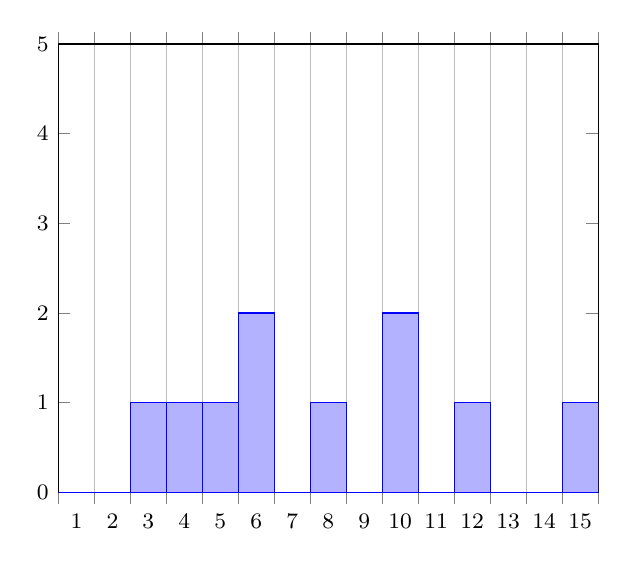
\begin{tikzpicture}
			\tikzstyle{every node}=[font=\footnotesize]
			\begin{axis}[ybar interval, ymin=0, ymax=5, xmin=1, xmax=16]
			\addplot coordinates {(1,0) (2,0) (3, 1) (4,1) (5,1) (6,2) (7,0) (8,1) (9,0) (10,2) (11,0) (12,1) (13,0) (14,0) (15,1) (16,0)};
			\end{axis}
		\end{tikzpicture}
		}
		\vspace{1cm}\\
		\textbf{Histograma de Sobrevivência Reincidência Tumor Sólido}
		\resizebox{300px}{!}{
		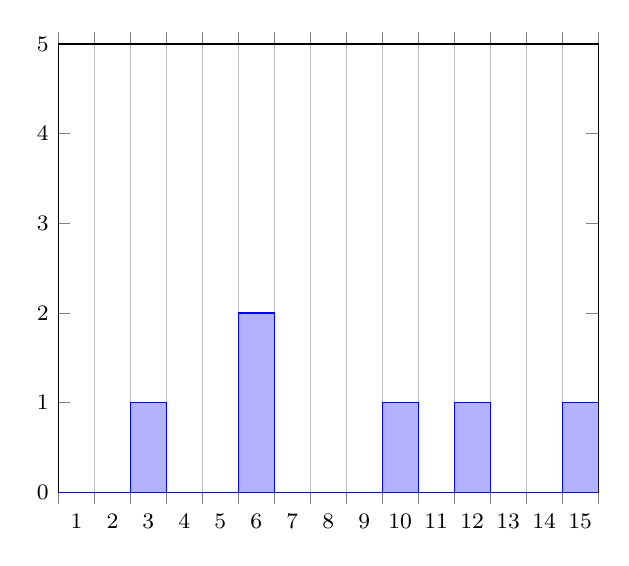
\begin{tikzpicture}
			\tikzstyle{every node}=[font=\footnotesize]
			\begin{axis}[ybar interval, ymin=0, ymax=5, xmin=1, xmax=16]
			\addplot coordinates {(1,0) (2,0) (3, 1) (4,0) (5,0) (6,2) (7,0) (8,0) (9,0) (10,1) (11,0) (12,1) (13,0) (14,0) (15,1) (16,0)};
			\end{axis}
		\end{tikzpicture}
		}
		\vspace{1cm}\\
		\textbf{Histograma de Censuras Reincidência Tumor Sólido}
		\resizebox{300px}{!}{
		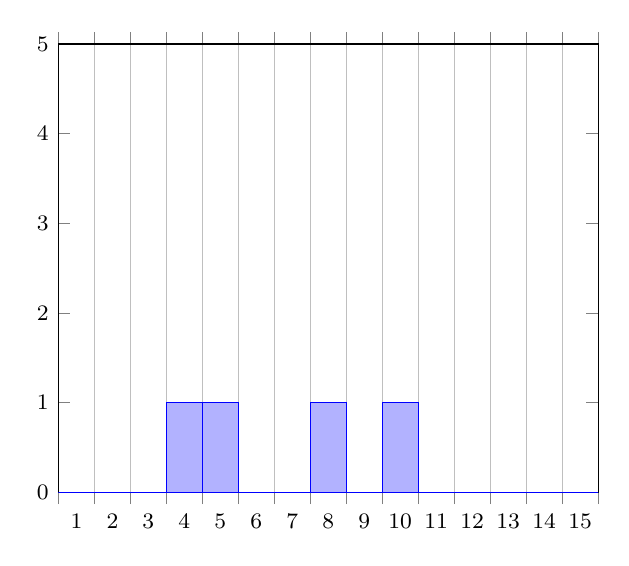
\begin{tikzpicture}
			\tikzstyle{every node}=[font=\footnotesize]
			\begin{axis}[ybar interval, ymin=0, ymax=5, xmin=1, xmax=16]
			\addplot coordinates {(1,0) (2,0) (3, 0) (4,1) (5,1) (6,0) (7,0) (8,1) (9,0) (10,1) (11,0) (12,0) (13,0) (14,0) (15,0) (16,0)};
			\end{axis}
		\end{tikzpicture}
		}
	\end{center}
	\vspace{1cm}
	O histograma embora apresente um pico, sugere uma razoável uniformidade das mortes ocasionada pela reincidência do tumor sólido, e variação no pico de reincidência ocorre dentro de um limite plausível, não excedendo uma reincidência do tumor sólido entre os pacientes entre meses consecutivos, excluindo-se o mês de pico de reincidência, em que houveram duas, já em termos do histograma dos eventos parece sugerir uma distribuição uniforme ou com uma ligeira concentração de eventos no meio do período. 
	\vspace{1cm}\\
	\textbf{2.2 Estimador de Kaplan-Meier}\\
	\begin{center}
		\resizebox{\linewidth}{!}{
		\begin{tabular}{ccccccc}\midrule
			\multicolumn{7}{c}{\textbf{Reincidência de Tumor Sólido}}\\ \midrule
			Tempo & Nº Risco & Eventos & Sobrevivência & Erro Padrão & IC$_{95\%}$ inferior & IC$_{95\%}$ superior\\ \midrule
			3.0 & 10 & 1 & 0.900 & 0.0949 & 0.7320 & 1\\ \midrule
			6.5 & 7 & 2 & 0.643 & 0.1679 & 0.3852 & 1\\ \midrule
			10.0 & 4 & 1 & 0.482 & 0.1877 & 0.2248 & 1\\ \midrule
			12.0 & 2 & 1 & 0.241 & 0.1946 & 0.0496 & 1\\ \midrule
			15.0 & 1 & 1 & 0.000 & 0.0000 & 0.0000 & 0\\ \midrule
		\end{tabular}
		}
		\vspace{1cm}\\
		\includegraphics[width=400px]{Gráfico 2.1.png}\\
	\end{center}
	\vspace{1cm}
	Apesar do formato escada do gráfico para a curva Kaplan-Meier é possível discernir uma tendência regular nos dados, outro ponto interessante é que o limite do intervalo de confiança superior para todo o escopo de análise é igual a 1, embora a taxa de sobrevivência tenha chegado a 0 após 15 semanas de estudo.\\ 
	\vspace{1cm}\\
	\textbf{2.2 Estimador de Nelson-Aalen}\\
	\vspace{1cm}\\
	\begin{center}
		\resizebox{\linewidth}{!}{
		\begin{tabular}{ccccccc}\midrule
			\multicolumn{7}{c}{\textbf{Reincidência de Tumor Sólido}}\\ \midrule
			Tempo & Nº Risco & Eventos & Sobrevivência & Erro Padrão & IC$_{95\%}$ inferior & IC$_{95\%}$ superior\\ \midrule
			3.0 & 10 & 1 & 0.905 & 0.0905 & 0.7438 & 1\\ \midrule
			6.5 & 7 & 2 & 0.664 & 0.1602 & 0.4138 & 1\\ \midrule
			10.0 & 4 & 1 & 0.517 & 0.1796 & 0.2617 & 1\\ \midrule
			12.0 & 2 & 1 & 0.314 & 0.1910 & 0.0951 & 1\\ \midrule
			15.0 & 1 & 1 & 0.115 & 0.1351 & 0.0116 & 1\\ \midrule
		\end{tabular}
		}
		\vspace{1cm}\\
		\includegraphics[width=400px]{Gráfico 2.2.png}\\
	\end{center}
	\vspace{1cm}
	Apesar de apresentar uma curva semelhante a Kaplan-Meier, o ajuste proposto pelo estimador Nelson-Aalen parece novamente capturar melhor o escopo dos dados já que obteve um Erro Padrão menor assim como um Intervalo de Confiança em relação a curva Kaplan-Meier. 
	\vspace{1cm}\\
	\textbf{2.3 Estimador Atuarial}
	\vspace{1cm}\\
	\begin{center}
	\resizebox{\linewidth}{!}{
		\begin{tabular}{ccccccccc}\midrule
			\multicolumn{9}{c}{\textbf{Reincidência de Tumor Sólido}}\\ \midrule
			Tempo & Sobreviventes & Censura & Nº Risco & Eventos & Sobrevivência & FdP  & Função Risco &  Erro Padrão\\ \midrule
			3-4 & 10 & 0 & 10.0 & 1 & 1.0000 & 0.1000 & 0.1053 & 0.0000\\ \midrule
			4-5.7 & 9 & 1 & 8.5 & 0 & 0.9000 & 0.0000 & 0.0000 & 0.0949\\ \midrule
			5.7-6.5 & 8 & 1 & 7.5 & 0 & 0.9000 & 0.0000 & 0.0000 & 0.0949\\ \midrule
			6.5-8.4 & 7 & 0 & 7.0 & 2 & 0.9000 & 0.1353 & 0.1754 & 0.0949\\ \midrule
			8.4-10 & 5 & 1 & 4.5 & 0 & 0.6429 & 0.0000 & 0.0000 & 0.1679\\ \midrule
			10-12 & 4 & 1 & 3.5 & 0 & 0.6429 & 0.0000 & 0.0000 & 0.1679\\ \midrule
			12-15 & 2 & 0 & 2.0 & 1 & 0.4592 & 0.0765 & 0.2222 & 0.1962\\ \midrule
			15-$\omega$ & 1 & 0 & 1.0 & 1 & 0.2296 & 0.000¨ & 0.000 & 0.1897
			\end{tabular}
			}
		\vspace{1cm}\\
		\includegraphics[width=400px]{Gráfico 2.3.png}\\
	\end{center}
	\vspace{1cm}
	A principal diferença observada na curva se sobrevivência atuarial para as demais é que os dados censurados são descartados por completo no cálculo da Função de Sobrevivência, assim mesmo ao final do estudo todos os pacientes, ou tenham sido censurados ou apresentaram reicidência do tumor sólido a função de sobrevivência é diferente de 0, nesse caso ficando próxima de 0,2 ao final do estudo. 
	\vspace{1cm}\\
	\textbf{2.5 Códigos do R}
	\vspace{1cm}\\
	library('survival')\\
	library('KMsurv')\\
	\vspace{0.25cm}\\
	\# Entrada dos dados\\
	tempos<- c(3,4,5.7,6.5,6.5,8.4,10,10,12,15)\\
	eventos<- c(1,0,0,1,1,0,1,0,1,1)\\
	\vspace{0.25cm}\\
	\# Estimador Kaplan-Meier\\
	ekm<-survfit(Surv(tempos,eventos)~1)\\
	summary(ekm)\\
	\vspace{0.25cm}\\
	\# Gráfico Kaplan-Meier\\
	plot(ekm, lty=1, xlab="Tempo (em Semanas)", ylab="S(t) estimada", main="Curva de Sobrevivência Kaplan-Meier de Reincidência do Tumor Sólido", conf.int=F)\\
	abline(h=0.5, col="red")\\
	legend(1, 0.3, lty=1, c("Tumor Sólido"), lwd=1, bty="n", cex=0.8)\\
	\vspace{0.25cm}\\
	\# Estimador Nelson-Aalen\\
	ena<-survfit(coxph(Surv(tempos,eventos)~1), method="breslow")\\
	summary(ena)\\
	\vspace{0.25cm}\\
	\# Gráfico Nelson-Aalen\\
	plot(ena, lty=1, main="Curva de Sobrevivência Nelson-Aalen de Reincidência do Tumor Sólido", xlab="Tempo (em semanas)", ylab="S(t) estimada", conf.int=FALSE)\\
	abline(h=0.5, col="red")\\
	legend(1, 0.3, lty=1, c("Tumor Sólido"), lwd=1, bty="n", cex=0.8)\\
	\vspace{0.25cm}\\
	\# Entrada dos dados\\
	intervalos<-c(3,4,5.7,6.5,8.4,10,12,15)\\
	reincidencia<-c(1,0,0,2,0,1,1,1)\\
	cens<-c(0,1,1,0,1,1,0,0)\\
	\vspace{0.25cm}\\
	\# Estimador Atuarial\\
	eac = lifetab(tis=intervalos, ninit=10, nlost=cens, nevent=reincidencia)
	round(eac, 4)\\
	\vspace{0.25cm}\\
	\# Gráfico Atuarial\\
	x<-rep(intervalos, rep(2,8))[1:15]\\
	x<-append(x, 0, 0)\\
	y<-rep(eac\$surv, rep(2,8))\\
	plot(x, y, type="l", lty=1, xlab="Tempo (em semanas)", ylab="S(t) estimada", xlim=c(0,15), ylim=c(0,1), main="Curva de Sobrevivência Atuarial de Reincidência de Tumor Sólido")\\
	abline(h=0.5, col="red")\\
	legend(1, 0.3, lty=1, c("Tumor Sólido"), lwd=1, bty="n", cex=0.8)\\
	\vspace{1cm}\\
	\textbf{3. Malária}
	\vspace{0.5cm}\\
	Um estudo experimental foi realizado com 44 camundongos para investigar a eficácia da imunização pela malária, o grupo 1 foi imunizado 30 dias antes do início do estudo, além disso, os grupos 1 e 3 também foram infectados com esquistossomose.
	\begin{center}
		\small{Tabela 3: Tempos de sobrevivência observados no estudo de imunização contra a malária.}\\
		\begin{tabular}{|c|c|c|}\hline
			\textbf{Grupos} & \textbf{n} & \textbf{Tempos de Sobrevivência (em Dias)}\\ \hline
			\textbf{1} & 16 & 7, 8, 8, 8, 8, 12, 12, 17, 18, 22, 30+, 30+, 30+, 30+, 30+, 30+\\ \hline
			\textbf{2} & 15 & 8, 8, 9, 10, 10, 14, 15, 15, 18, 19, 21, 22, 22, 23, 25\\ \hline
			\textbf{3} & 13 & 8, 8, 8, 8, 8, 8, 9, 10, 10, 10, 11, 17, 19\\ \hline
		\end{tabular}
	\end{center}
	\vspace{1cm}
	\textbf{3.1 Histograma dos dados}
	\begin{center}
		\vspace{1cm}
		\textbf{Histograma de Eventos Comundongos Infectados por Malária Grupo 1}
		\resizebox{350px}{!}{
			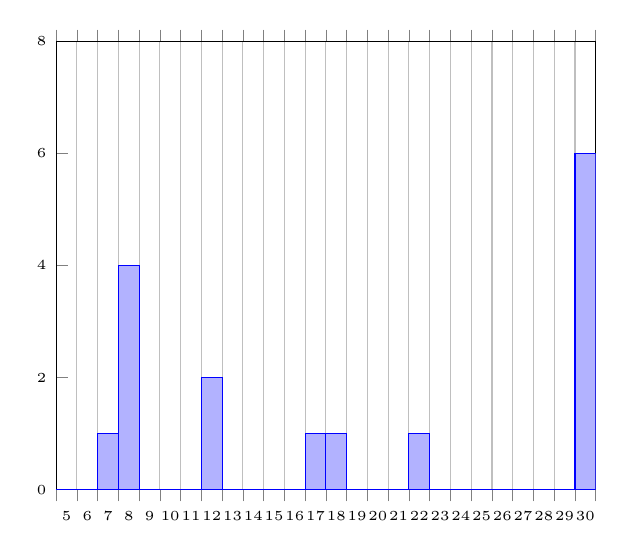
\begin{tikzpicture}
			\tikzstyle{every node}=[font=\tiny]
			\begin{axis}[ybar interval, ymin=0, ymax=8, xmin=5, xmax=31]
			\addplot coordinates {(5,0) (6,0) (7,1) (8,4) (9,0) (10,0) (11,0) (12,2) (13,0) (14,0) (15,0) (16,0) (17,1) (18,1) (19,0) (20,0) (21,0) (22,1) (23,0) (24,0) (25,0) (26,0) (27,0) (28,0) (29,0) (30,6) (31,0)};
			\end{axis}	
			\end{tikzpicture}
		}
		\vspace{1cm}\\
		\textbf{Histograma de Sobrevivência Comundongos Infectados por Malária Grupo 1}
		\resizebox{350px}{!}{
		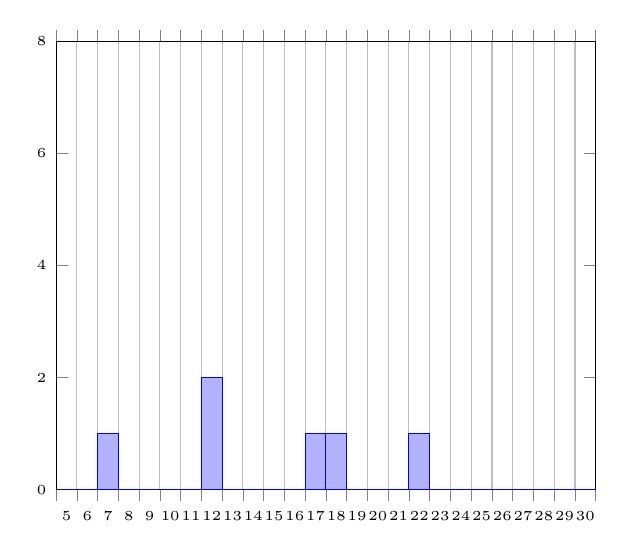
\begin{tikzpicture}
			\tikzstyle{every node}=[font=\tiny]
			\begin{axis}[ybar interval, ymin=0, ymax=8, xmin=5, xmax=31]
			\addplot coordinates {(5,0) (6,0) (7,1) (8,0) (9,0) (10,0) (11,0) (12,2) (13,0) (14,0) (15,0) (16,0) (17,1) (18,1) (19,0) (20,0) (21,0) (22,1) (23,0) (24,0) (25,0) (26,0) (27,0) (28,0) (29,0) (30,0) (31,0)};
			\end{axis}	
		\end{tikzpicture}
		}
		\vspace{1cm}\\
		\textbf{Histograma de Censuras Comundongos Infectados por Malária Grupo 1}
		\resizebox{350px}{!}{
		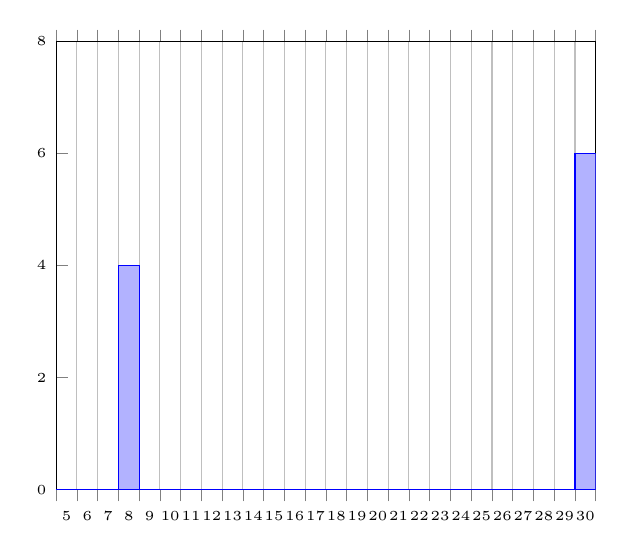
\begin{tikzpicture}
			\tikzstyle{every node}=[font=\tiny]
			\begin{axis}[ybar interval, ymin=0, ymax=8, xmin=5, xmax=31]
			\addplot coordinates {(5,0) (6,0) (7,0) (8,4) (9,0) (10,0) (11,0) (12,0) (13,0) (14,0) (15,0) (16,0) (17,0) (18,0) (19,0) (20,0) (21,0) (22,0) (23,0) (24,0) (25,0) (26,0) (27,0) (28,0) (29,0) (30,6) (31,0)};
			\end{axis}	
		\end{tikzpicture}
		}
		\vspace{1cm}\\
		\textbf{Histograma de Sobrevivência Comundongos Infectados por Malária Grupo 2}
		\resizebox{350px}{!}{
		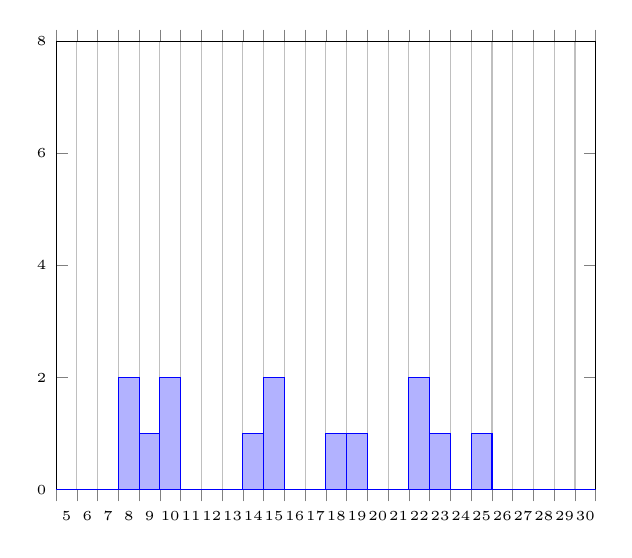
\begin{tikzpicture}
			\tikzstyle{every node}=[font=\tiny]
			\begin{axis}[ybar interval, ymin=0, ymax=8, xmin=5, xmax=31]
			\addplot coordinates {(5,0) (6,0) (7, 0) (8,2) (9,1) (10,2) (11,0) (12,0) (13,0) (14,1) (15,2) (16,0) (17,0) (18,1) (19,1) (20,0) (21,0) (22,2) (23,1) (24,0) (25,1) (26,0) (27,0) (28,0) (29,0) (30,0) (31,0)};
			\end{axis}	
		\end{tikzpicture}
		}
	\vspace{1cm}\\
	\textbf{Histograma de Sobrevivência Comundongos Infectados por Malária Grupo 3}
	\resizebox{350px}{!}{
		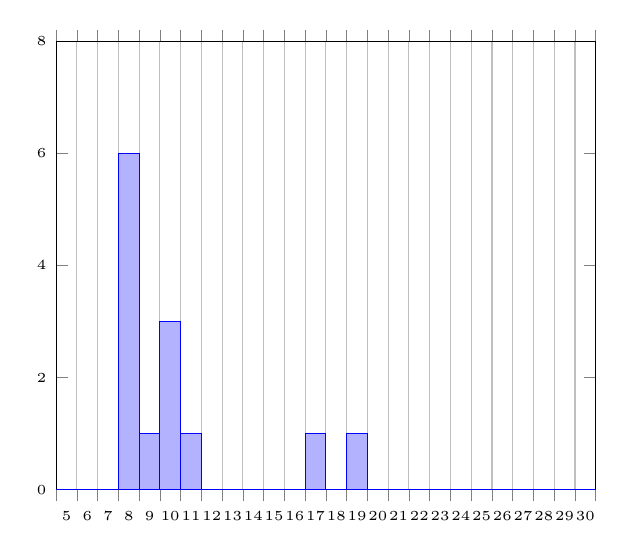
\begin{tikzpicture}
			\tikzstyle{every node}=[font=\tiny]
			\begin{axis}[ybar interval, ymin=0, ymax=8, xmin=5, xmax=31]
			\addplot coordinates {(5,0) (6,0) (7, 0) (8,6) (9,1) (10,3) (11,1) (12,0) (13,0) (14,0) (15,0) (16,0) (17,1) (18,0) (19,1) (20,0) (21,0) (22,0) (23,0) (24,0) (25,0) (26,0) (27,0) (28,0) (29,0) (30,0) (31,0)};
			\end{axis}	
		\end{tikzpicture}
	}
	\end{center}
	\vspace{1cm}
	Os histoogramas de sobrevivência dos grupos 1 e 3 indicam um pico na mortalidade dos indivíduos uma semana, oitavo dia, após início do estudo que vai estabilizando em níveis mais baixos nos dias posteriores, já no grupo 2 apresenta uma taxa quase constante ao longo de todo o período de estudo, tendo uma variação de no máximo duas mortes entres dias consecutivos, é interessante ressaltar que os dados são mais fidedignos nesse estudo pelo baixo índice censura, e apenas do II, observada apenas no grupo 1.
	\vspace{1cm}\\
	\textbf{3.2.1 Estimador Kaplan-Meier}
	\vspace{1cm}\\
	\begin{center}
		\resizebox{\linewidth}{!}{
		\begin{tabular}{ccccccc}\midrule
			\multicolumn{7}{c}{\textbf{Grupo 1}}\\ \midrule 
			Tempo & Nº Risco & Eventos & Sobrevivência & Erro Padrão & IC$_{95\%}$ inferior & IC$_{95\%}$ superior\\ \midrule
			7 & 16 & 1 & 0.938 & 0.0605 & 0.826 & 1.000\\ \midrule
			8 & 15 & 4 & 0.688 & 0.1159 & 0.494 & 0.957\\ \midrule
			12 & 11 & 2 & 0.562 & 0.1240 & 0.365 & 0.867\\ \midrule
			17 & 9 & 1 & 0.500 & 0.1250 & 0.306 & 0.816\\ \midrule
			18 & 8 & 1 & 0.438 & 0.1240 & 0.251 & 0.763\\ \midrule
			22 & 7 & 1 & 0.375 & 0.1210 & 0.199 & 0.706\\ \midrule
		\end{tabular}
		}
		\vspace{1cm}\\
		\resizebox{\linewidth}{!}{
		\begin{tabular}{ccccccc}\midrule
			\multicolumn{7}{c}{\textbf{Grupo 2}}\\ \midrule 
			Tempo & Nº Risco & Eventos & Sobrevivência & Erro Padrão & IC$_{95\%}$ inferior & IC$_{95\%}$ superior\\ \midrule 
		   	8 & 15 & 2 & 0.8667 & 0.0878 & 0.7106 & 1.000\\ \midrule
			9 & 13 & 1 & 0.8000 & 0.1033 & 0.6212 & 1.000\\ \midrule
			10 & 12 & 2 & 0.6667 & 0.1217 & 0.4661 & 0.953\\ \midrule
			14 & 10 & 1 & 0.6000 & 0.1265 & 0.3969 & 0.907\\ \midrule
			15 & 9 & 2 & 0.4667 & 0.1288 & 0.2717 & 0.802\\ \midrule
			18 & 7 & 1 & 0.4000 & 0.1265 & 0.2152 & 0.743\\ \midrule
			19 & 6 & 1 & 0.3333 & 0.1217 & 0.1630 & 0.682\\ \midrule
			21 & 5 & 1 & 0.2667 & 0.1142 & 0.1152 & 0.617\\ \midrule
			22 & 4 & 2 & 0.1333 & 0.0878 & 0.0367 & 0.484\\ \midrule
			23 & 2 & 1 & 0.0667 & 0.0644 & 0.0100 & 0.443\\ \midrule
			25 & 1 & 1 & 0.0000 & 0.0000 & 0.0000 & 0.000\\ \midrule
		\end{tabular}
		}
		\vspace{1cm}\\
		\resizebox{\linewidth}{!}{
		\begin{tabular}{ccccccc}\midrule
			\multicolumn{7}{c}{\textbf{Grupo 3}}\\ \midrule 
			Tempo & Nº Risco & Eventos & Sobrevivência & Erro Padrão & IC$_{95\%}$ inferior & IC$_{95\%}$ superior\\ \midrule
			8 & 13 & 6 & 0.5385 & 0.1383 & 0.3255 & 0.891\\ \midrule
			9 & 7 & 1 & 0.4615 & 0.1383 & 0.2566 & 0.830\\ \midrule
			10 & 6 & 3 & 0.2308 & 0.1169 & 0.0855 & 0.623\\ \midrule
			11 & 3 & 1 & 0.1538 & 0.1001 & 0.0430 & 0.550\\ \midrule
		\end{tabular}
		}
		\vspace{1cm}\\
		\includegraphics[width=400px]{Gráfico 3.1.png}\\
	\end{center}
	\vspace{1cm}
	As Curvas de Sobrevivência começam a apresentar as primeiras falhas por volta do mesmo tempo 7-8 dias, mas a frequência dos eventos entre os grupos impacta diretamente ao final do estudo, em que o grupo 1 que foi imunizado é o único que ocorre censura pois os indivíduos vivem além do escopo de tempo que o estudo se propôs, o grupo 2 se aproxima de 0 em taxa de sobrevivência por volta do dia 25, enquanto o grupo 3, ocorre de maneira similar, mas por volta dia 18.
	\vspace{1cm}\\
	\textbf{3.2.2 Teste Logrank para Curvas de Sobrevida Kaplan-Meier}
	\vspace{0.5cm}\\
	\begin{center}
		\resizebox{\linewidth}{!}{
		\begin{tabular}{cccccc}\midrule
			& Elementos & Observado & Esperado & $\dfrac{(O-E)^{2}}{E}$ & $\dfrac{(O-E)^{2}}{\sigma}$\\ \midrule
			grupo=1 & 16 & 10 & 17.00 & 2.8816 & 6.4111\\ \midrule
			grupo=2 & 15 & 15 & 14.51 & 0.0167 & 0.0317\\ \midrule
			grupo=3 & 13 & 13 & 6.49 & 6.5190 & 10.4447\\ \midrule
			\multicolumn{6}{c}{Chi-Quadrado = 12.6  com 2 grau de liberdade, p= 0.002}\\ \midrule
		\end{tabular}
		}
		\vspace{1cm}\\
		\resizebox{\linewidth}{!}{
		\begin{tabular}{cccccc}\midrule
			& Elementos & Observado & Esperado & $\dfrac{(O-E)^{2}}{E}$ & $\dfrac{(O-E)^{2}}{\sigma}$\\ \midrule
			grupo=1 & 16 & 10 & 13.7 & 1.01 & 2.53\\ \midrule
			grupo=2 & 15 & 15 & 11.3 & 1.23 & 2.53\\ \midrule
			\multicolumn{6}{c}{Chi-Quadrado = 2.5  com 1 grau de liberdade, p= 0.1}\\ \midrule
		\end{tabular}
		}
		\vspace{1cm}\\
		\resizebox{\linewidth}{!}{
		\begin{tabular}{cccccc}\midrule
			& Elementos & Observado & Esperado & $\dfrac{(O-E)^{2}}{E}$ & $\dfrac{(O-E)^{2}}{\sigma}$\\ \midrule
			grupo=2 & 15 & 15 & 20.53 & 1.49 & 7.98\\ \midrule
			grupo=3 & 13 & 13 & 7.47 & 4.08 & 7.98\\ \midrule
			\multicolumn{6}{c}{Chi-Quadrado = 8  com 1 grau de liberdade, p= 0.005}\\ \midrule
		\end{tabular}
		}
		\vspace{1cm}\\
		\resizebox{\linewidth}{!}{
		\begin{tabular}{cccccc}\midrule
			& Elementos & Observado & Esperado & $\dfrac{(O-E)^{2}}{E}$ & $\dfrac{(O-E)^{2}}{\sigma}$\\ \midrule
			grupo=1 & 16 & 10 & 15.34 & 1.86 & 7.86\\ \midrule
			grupo=3 & 13 & 13 & 7.66 & 3.72 & 7.86\\ \midrule
			\multicolumn{6}{c}{Chi-Quadrado = 7.9  com 1 grau de liberdade, p= 0.005}\\ \midrule		
		\end{tabular}
		}
	\end{center}
	\vspace{1cm}
	A partir do Teste Logrank dos Estimadores de Kaplan-Meier podemos concluir que não podemos rejeitar a Hipótese Nula de que as curvas do grupo 1 e do grupo 2 sigam a mesma distribuição, mas devemos rejeitar H$_{0}$ no caso entre os grupos 1 e 3, e os grupos 2 e 3.
	\vspace{1cm}\\
	\textbf{3.3 Estimador de Nelson-Aalen}
	\vspace{1cm}\\
	\begin{center}
		\resizebox{\linewidth}{!}{
		\begin{tabular}{ccccccc}\midrule
			\multicolumn{7}{c}{\textbf{Imunização Contra Malária - Grupo 1}}\\ \midrule
			Tempo & Nº Risco & Eventos & Sobrevivência & Erro Padrão & IC$_{95\%}$ inferior & IC$_{95\%}$ superior\\ \midrule
			7 & 15 & 1 & 0.936 & 0.0624 & 0.821 & 1.000\\ \midrule
			8 & 14 & 4 & 0.703 & 0.1108 & 0.516 & 0.958\\ \midrule
			12 & 10 & 2 & 0.576 & 0.1219 & 0.380 & 0.872\\ \midrule
			17 & 8 & 1 & 0.508 & 0.1249 & 0.314 & 0.823\\ \midrule
			18 & 7 & 1 & 0.440 & 0.1252 & 0.252 & 0.769\\ \midrule
			22 & 6 & 1 & 0.373 & 0.1229 & 0.195 & 0.711\\ \midrule
		\end{tabular}
		}
		\vspace{1cm}\\
		\resizebox{\linewidth}{!}{
		\begin{tabular}{ccccccc}\midrule
			\multicolumn{7}{c}{\textbf{Imunização Contra Malária - Grupo 2}}\\ \midrule
			Tempo & Nº Risco & Eventos & Sobrevivência & Erro Padrão & IC$_{95\%}$ inferior & IC$_{95\%}$ superior\\ \midrule
			8 & 16 & 2 & 0.961 & 22.3 & 1.77e-20 & 1\\ \midrule
			9 & 14 & 1 & 0.940 & 34.4 & 7.14e-32 & 1\\ \midrule
			10 & 13 & 2 & 0.895 & 58.6 & 1.46e-56 & 1\\ \midrule
			14 & 11 & 1 & 0.868 & 72.0 & 2.24e-71 & 1\\ \midrule
			15 & 10 & 2 & 0.813 & 98.9 & 2.70e-104 & 1\\ \midrule
			18 & 8 & 1 & 0.780 & 114.1 & 1.86e-125 & 1\\ \midrule
			19 & 7 & 1 & 0.742 & 130.2 & 3.80e-150 & 1\\ \midrule
			21 & 6 & 1 & 0.700 & 147.0 & 8.97e-180 & 1\\ \midrule
			22 & 5 & 2 & 0.603 & 179.3 & 7.68e-254 & 1\\ \midrule
			23 & 3 & 1 & 0.521 & 199.9 & 0.00e+00 & 1\\ \midrule
			25 & 2 & 1 & 0.387 & 216.1 & 0.00e+00 & 1\\ \midrule
		\end{tabular}
		}
		\vspace{1cm}\\
		\resizebox{\linewidth}{!}{
		\begin{tabular}{ccccccc}\midrule
			\multicolumn{7}{c}{\textbf{Imunização Contra Malária - Grupo 3}}\\ \midrule
			Tempo & Nº Risco & Eventos & Sobrevivência & Erro Padrão & C$_{95\%}$ inferior & IC$_{95\%}$ superior\\ \midrule
			8 & 13 & 6 & 0.630 & 0.1188 & 0.4357 & 0.912\\ \midrule
			9 & 7 & 1 & 0.546 & 0.1292 & 0.3438 & 0.869\\ \midrule
			10 & 6 & 3 & 0.331 & 0.1237 & 0.1595 & 0.689\\ \midrule
			11 & 3 & 1 & 0.237 & 0.1188 & 0.0891 & 0.633\\ \midrule
			17 & 2 & 1 & 0.144 & 0.1019 & 0.0360 & 0.576\\ \midrule
			19 & 1 & 1 & 0.053 & 0.0649 & 0.0048 & 0.585\\ \midrule
		\end{tabular}
		}
		\vspace{1cm}\\
		\includegraphics[width=400px]{Gráfico 3.2.png}\\
	\end{center}
	\vspace{1cm}
	Embora inicialmente as curvas referentes ao grupo 1 e grupo 3 se assemelhem, sendo a curva do grupo 2 destoante, ao longo do estudo a curva do grupo 1 vai se aproximando da curva observado no grupo 2, assim ao final do processo a curva destoante das demais é a do grupo 3, que se aproxima de 0 taxa de sobrevivência por volta dia 19, enquanto as demais terminam o estudo próximas a 0,4 de sobrevivência. 
	\vspace{1cm}\\
	\textbf{3.4 Estimador Atuarial}
	\vspace{1cm}
	\begin{center}
		\resizebox{\linewidth}{!}{
		\begin{tabular}{ccccccccc}\midrule
			\multicolumn{9}{c}{\textbf{Imunização Contra Malária - Grupo 1}}\\ \midrule
			Tempo & Sobreviventes & Censura & Nº Risco & Eventos & Sobrevivência & FdP  & Função Risco &  Erro Padrão\\ \midrule
			7-8 & 16 & 0 & 16 & 1 & 1.0000 & 0.0625 & 0.0645 & 0.0000\\ \midrule
			8-12 & 15 & 0 & 15 & 4 & 0.9375 & 0.0625 & 0.0769 & 0.0605\\ \midrule
		12-17 & 11 & 0 & 11 & 2 & 0.6875 & 0.0250 & 0.0400 & 0.1159\\ \midrule
		17-18 & 9 & 0 & 9 & 1 & 0.5625 & 0.0625 & 0.1176 & 0.1240\\ \midrule
		18-22 & 8 & 0 & 8 & 1 & 0.5000 & 0.0156 & 0.0333 & 0.1250\\ \midrule
		22-30 & 7 & 0 & 7 & 1 & 0.4375 & 0.0078 & 0.0192 & 0.1240\\ \midrule
		30-$\omega$ & 6 & 6 & 3 & 0 & 0.3750 & 0.0000 & 0.0000 & 0.1210\\ \midrule
		\end{tabular}
		}
		\vspace{1cm}\\
		\resizebox{\linewidth}{!}{
		\begin{tabular}{ccccccccc}\midrule
			\multicolumn{9}{c}{\textbf{Imunização Contra Malária - Grupo 2}}\\ \midrule
			Tempo & Sobreviventes & Censura & Nº Risco & Eventos & Sobrevivência & FdP  & Função Risco &  Erro Padrão\\ \midrule
			8-9 & 15 & 0 & 15 & 2 & 1.0000 & 0.1333 & 0.1429 & 0.0000\\ \midrule
			9-10 & 13 & 0 & 13 & 1 & 0.8667 & 0.0667 & 0.0800 & 0.0878\\ \midrule 
			10-14 & 12 & 0 & 12 & 2 & 0.8000 & 0.0333 & 0.0455 & 0.1033\\ \midrule 
			14-15 & 10 & 0 & 10 & 1 & 0.6667 & 0.0667 & 0.1053 & 0.1217\\ \midrule 
			15-18 & 9 & 0 & 9 & 2 & 0.6000 & 0.0444 & 0.0833 & 0.1265\\ \midrule 
			18-19 & 7 & 0 & 7 & 1 & 0.4667 & 0.0667 & 0.1538 & 0.1288 \\ \midrule
			19-21 & 6 & 0 & 6 & 1 & 0.4000 & 0.0333 & 0.0909 & 0.1265\\ \midrule 
			21-22 & 5 & 0 & 5 & 1 & 0.3333 & 0.0667 & 0.2222 & 0.1217\\ \midrule 
			22-23 & 4 & 0 & 4 & 2 & 0.2667 & 0.1333 & 0.6667 & 0.1142\\ \midrule
			23-25 & 2 & 0 & 2 & 1 & 0.1333 & 0.0333 & 0.3333 & 0.0878\\ \midrule
			25-$\omega$ & 1 & 0 & 1 & 1 & 0.0667 & 0.000 & 0.0000 & 0.0644\\ \midrule    
		\end{tabular}
		}
		\vspace{1cm}\\
		\resizebox{\linewidth}{!}{
		\begin{tabular}{ccccccccc}\midrule
			\multicolumn{9}{c}{\textbf{Imunização Contra Malária - Grupo 3}}\\ \midrule
			Tempo & Sobreviventes & Censura & Nº Risco & Eventos & Sobrevivência & FdP  & Função Risco &  Erro Padrão\\ \midrule
			8-9 & 13 & 0 & 13 & 6 & 1.0000 & 0.4615 & 0.6000 & 0.0000\\ \midrule
			9-10 & 7 & 0 & 7 & 1 & 0.5385 & 0.0769 & 0.1538 & 0.1383\\ \midrule
			10-11 & 6 & 0 & 6 & 3 & 0.4615 & 0.2308 & 0.6667 & 0.1383\\ \midrule
			11-17 & 3 & 0 & 3 & 1 & 0.2308 & 0.0128 & 0.0667 & 0.1169\\ \midrule
			17-19 & 2 & 0 & 2 & 1 & 0.1538 & 0.0385 & 0.3333 & 0.1001\\ \midrule
			19-$\omega$ & 1 & 0 & 1 & 1 & 0.0769 & 0.000 & 0.000 & 0.0739\\ \midrule
		\end{tabular}
		}
		\vspace{1cm}\\
		\includegraphics[width=400px]{Gráfico 3.3.png}\\
	\end{center}
	\vspace{1cm}
	A curva de sobrevivência pelo método atuarial produziu os gráficos com maior distinção entre os 3 grupos analisados. Embora a curva do grupo 1 e do grupo 2 tenham sido similar ao longo grande parte do estudo a partir do dia 20 elas se distanciaram, em que o grupo 1 teve uma sobrevivência próxima a 0,4, enquanto o grupo 3, chegou próxima de zero no dia 23, o que também aconteceu com o grupo 2, mas em um período bem anterior, no dia 18.
	\vspace{1cm}\\
	\textbf{3.5 Códigos do R}
	\vspace{1cm}\\
	\# Importando bibliotecas\\
	library('survival')\\
	library('KMsurv')\\
	\vspace{0.25cm}\\
	\# Entrada dos dados\\
	tempos<-c(7,8,8,8,8,12,12,17,18,22,30,30,30,30,30,30,8,8,9,10,10,14,15,15,18,19,21,22,22,23,25,8,8,8,8,8,8,9,10,10,10,11,17,19)\\
	eventos<-c(rep(1,10), rep(0,6), rep(1,15), rep(1,13))\\
	grupo<-c(rep(1,16), rep(2,15), rep(3,13))\\
	\vspace{0.25cm}\\
	\# Estimador Kaplan-Meier\\
	ekm<-survfit(Surv(tempos,eventos)~grupo)\\
	summary(ekm)\\
	\vspace{0.25cm}\\
	\# Gráfico Kaplan-Meier\\
	plot(ekm, lty=c(1,4,2), main="Curva de Sobrevivência Kaplan-Meier dos Camundogos Infectados com Malária", xlab="Tempo (em dias)", ylab="S(t) estimada", mark.time=T)\\
	abline(h=0.5, col="red")\\
	legend(1, 0.3, lty=c(1,4,2), c("Grupo 1","Grupo 2","Grupo 3"), lwd=1, bty="n", cex=0.8)\\
	\vspace{0.25cm}\\
	\# Log-rank estimador Kaplan-Meier\\
	survdiff(Surv(tempos,eventos)~grupo, rho=0)\\
	survdiff(Surv(tempos[1:31],eventos[1:31])~grupo[1:31], rho=0)\\
	survdiff(Surv(tempos[17:44],eventos[17:44])~grupo[17:44], rho=0)\\
	survdiff(Surv(c(tempos[1:16],tempos[32:44]),c(eventos[1:16],eventos[32:44]))~c(grupo[1:16],grupo[32:44]), rho=0)\\
	\vspace{0.25cm}\\
	\# Estimador Nelson-Aalen\\
	ena.g1<-survfit(coxph(Surv(tempos[1:15],eventos[1:15])~grupo[1:15]), type="breslow")\\
	summary(ena.g1)\\
	ena.g2<-survfit(coxph(Surv(tempos[16:31],eventos[16:31])~grupo[16:31]), type="breslow")\\
	summary(ena.g2)\\
	ena.g3<-survfit(coxph(Surv(tempos[32:44],eventos[32:44])~grupo[32:44]), type="breslow")\\
	summary(ena.g3)\\
	\vspace{0.25cm}\\
	\# Gráfico Nelson-Aalen\\
	plot(ena.g1, lty=1, main="Curva de Sobrevivência Nelson-Aalen dos Camundogos Infectados com Malária", xlab="Tempo (em Dias)", ylab="S(t) estimada")\\
	abline(h=0.5, col="red")\\
	par(new=TRUE)\\
	plot(ena.g2, lty=4, xlab="Tempo (em dias)", ylab="S(t) estimada", conf.int=FALSE)\\
	par(new=TRUE)\\
	plot(ena.g3, lty=2, xlab="Tempo (em dias)", ylab="S(t) estimada", conf.int=FALSE)\\
	legend(1, 0.3, lty=c(1,4,2), c("Grupo 1","Grupo 2","Grupo 3"), lwd=1, bty="n", cex=0.8)\\
	\vspace{0.25cm}\\
	\# Entrada dos dados\\
	intervalos<-c(7,8,12,17,18,22,30,8,9,10,14,15,18,19,21,22,23,25,8,9,10,11,17,19)\\
	mortes<-c(1,4,2,1,1,1,0,2,1,2,1,2,1,1,1,2,1,1,6,1,3,1,1,1)\\
	cens<-c(rep(0,6),6,rep(0,17))\\
	\vspace{0.25cm}\\
	\# Estimador Atuarial\\
	eac.g1 = lifetab(tis=intervalos[1:7], ninit=16, nlost=cens[1:7], nevent=mortes[1:7])\\
	round(eac.g1, 4)\\
	eac.g2 = lifetab(tis=intervalos[8:18], ninit=15, nlost=cens[8:18], nevent=mortes[8:18])\\
	round(eac.g2, 4)\\
	eac.g3 = lifetab(tis=intervalos[19:24], ninit=13, nlost=cens[19:24], nevent=mortes[19:24])\\
	round(eac.g3, 4)\\
	\vspace{0.25cm}\\
	\# Gráfico Atuarial\\
	x1<-rep(intervalos[1:7], rep(2,7))[1:13]\\
	x1<-append(x1, 0, 0)\\
	y1<-rep(eac.g1\$surv, rep(2,7))\\
	plot(x1, y1, type="l", lty=1, xlab="Tempo (em semanas)", ylab="S(t) estimada", xlim=c(0,30), ylim=c(0,1), main="Curva de Sobrevivência Atuarial dos Pacientes no Tratamento de Hepatite")\\
	abline(h=0.5, col="red")\\
	x2<-rep(intervalos[8:18], rep(2,11))[1:21]\\
	x2<-append(x2, 0, 0)\\
	y2<-rep(eac.g2\$surv, rep(2,11))\\
	par(new=TRUE)\\
	plot(x2, y2, type="l", lty=4,  xlab="Tempo (em semanas)", ylab="S(t) estimada", xlim=c(0,30), ylim=c(0,1))\\
	x3<-rep(intervalos[19:24], rep(2,6))[1:11]\\
	x3<-append(x3, 0, 0)\\
	y3<-rep(eac.g3\$surv, rep(2,6))\\
	par(new=TRUE)\\
	plot(x3, y3, type="l", lty=2,  xlab="Tempo (em semanas)", ylab="S(t) estimada", xlim=c(0,30), ylim=c(0,1))\\
	legend(1, 0.3, lty=c(1,4,2), c("Grupo 1","Grupo 2","Grupo 3"), lwd=1, bty="n", cex=0.8)\\
\end{document}
